\newpage

\section{Ricerca informata}

Che differenza c'è tra ricerca non informata e informata?

Nella ricerca informata si ha più conoscenza del problema e si
velocizza il processo di ricerca.

Sia f la funzione di valutazione di costo.

La funzione h(n) è una euristica ed è un componente di f.

h(n): costo stimato del percorso più economico dal nodo n allo stato
obiettivo (goal)

h(n) dipende solo dallo stato associato a n.
Assunzioni: $h(n) >= 0 \land h(n) = 0$ $\forall n$ all'inizio.

\subsection{Uniform Cost Search - richiami}
Espande il nodo con il minore costo di cammino g(n), ma in questo caso \dots

g(n) nella uniform cost search fornisce il costo per andare dallo stato
iniziale (root) fino ad n g(n) non è una stima, ma un costo certo.

f(n) = h(n)

La versione della ricerca su grafo è più furba (non rivisita stati già esplorati)
rispetto a quella su albero. 

\subsection{Best first seach}
Espande il nodo che è più vicino all'obiettivo tra i nodi collegati al corrente.
Ogni nodo deve sapere quanto è distante dal nodo obiettivo.

Completo? No, può ciclare o arrivare in un punto morto oppure c'è un infinito.
numero di stati.

Ottimo? No, dà una soluzione greedy

\subsection{A* algorithm}
f(n) = g(n) + h(n)
g(n) = costo già sostenuto prima da stato iniziale al nodo n (costo effettivo fatto)
h(n) = costo da n a stato obiettivo (euristica)

Completo? Sì.

Complessità? Esponenziale.

Ottimo? Sì, (a certe condizioni) vedi il teorema\dots

\subsection{Euristica ammissibile}

Un'euristica è ammissibile se vale: $h(n) <= h^*(n)$
(cioè non deve sovrastimare il costo per raggiungere un obiettivo)

\textbf{Teorema su A*}
Se h(n) è un'euristica ammissibile,  A* usando la ricerca su albero è ottimale.
Dimostrazione - Si basa sul confronto di f e g tra un ottimo G e un sub-ottimo G2

\subsection{Euristica consistente}

Un'euristica è consistente se:
$\forall n \land \forall succ(n) = n'$ generato da un'azione act vale:
$h(n) <= c(n,act,n') + h(n')$
dove c(n,act,n') è il costo per andare da n a n' con l'azione act.

Se un'euristica è consistente allora è anche ammissibile.
Questa implicazione (Consistenza $\rightarrow$ Ammissibilità) si dimostra per
induzione su uno stato n

Caso base:
h(g) = 0.

Sia n un genitore di G.

h(n) = c(n,a,g) + h(g) = c(n,a,g) = h*(n) quindi h(n) <= h*(n) ammissibile.

\subsection{Euristiche e dominanza}

Un'euristica h2 domina un'euristica h1 se $h2(n) >= h1(n) \forall n$ .

Un problema rilassato ha meno vincoli rispetto all'originale.
Grafo del problema rilassato = Supergrafo problema originale.

\subsection{Ricerca locale}

Gli algoritmi di ricerca locale esplorano uno spazio degli stati che può avere
una forma simile a quella in figura \ref{img:landscape}

\begin{figure}[H]
\centering
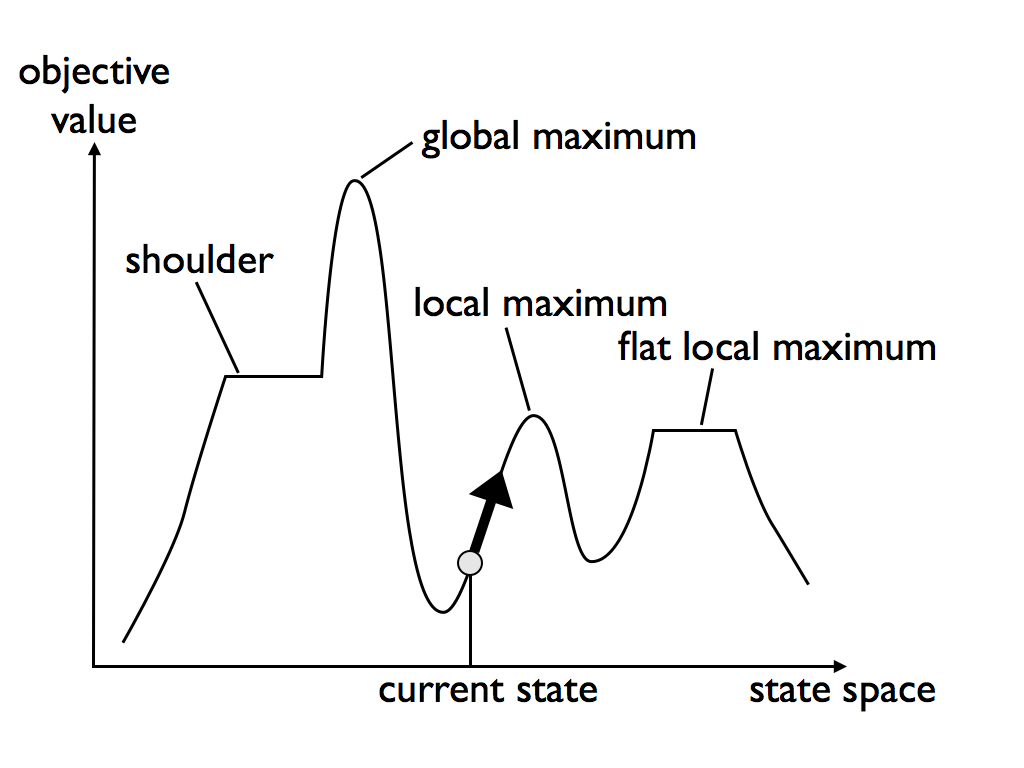
\includegraphics[width=0.4\textwidth]{landscape}
\caption{Esempio di uno spazio degli stati a 1 dimensione definito da una
funzione obiettivo}
\label{fig:landscape}
\end{figure}

Lo spazio degli stati ha delle locazioni (ascisse) e delle elevazioni
(valori delle ordinate).

Se l'elevazione corrisponde a un costo, occorre cercare un minimo globale,
se corrisponde a un ricavo di qualche tipo, occorre cercare un massimo globale.

Gli algoritmi di ricerca locale possono essere \textbf{completi} (trovano
sempre lo stato obiettivo se esiste) oppure \textbf{ottimali} (riescono sempre a
trovare un massimo e un minimo globale)
